%%%%%%%%%%%%%%%%%%%%%%%%%%%%%%%%%%%%%%%%%
% Beamer Presentation
% LaTeX Template
% Version 1.0 (10/11/12)
%
% This template has been downloaded from:
% http://www.LaTeXTemplates.com
%
% License:
% CC BY-NC-SA 3.0 (http://creativecommons.org/licenses/by-nc-sa/3.0/)
%
%%%%%%%%%%%%%%%%%%%%%%%%%%%%%%%%%%%%%%%%%

%----------------------------------------------------------------------------------------
%	PACKAGES AND THEMES
%----------------------------------------------------------------------------------------

\documentclass{beamer}

\mode<presentation> {

% The Beamer class comes with a number of default slide themes
% which change the colors and layouts of slides. Below this is a list
% of all the themes, uncomment each in turn to see what they look like.

%\usetheme{default}
%\usetheme{AnnArbor}
%\usetheme{Antibes}
%\usetheme{Bergen}
%\usetheme{Berkeley}
%\usetheme{Berlin}
%\usetheme{Boadilla}
%\usetheme{CambridgeUS}
%\usetheme{Copenhagen}
\usetheme{Darmstadt}
%\usetheme{Dresden}
%\usetheme{Frankfurt}
%\usetheme{Goettingen}
%\usetheme{Hannover}
%\usetheme{Ilmenau}
%\usetheme{JuanLesPins}
%\usetheme{Luebeck}
%\usetheme{Madrid}
%\usetheme{Malmoe}
%\usetheme{Marburg}
%\usetheme{Montpellier}
%\usetheme{PaloAlto}
%\usetheme{Pittsburgh}
%\usetheme{Rochester}
%\usetheme{Singapore}
%\usetheme{Szeged}
%\usetheme{Warsaw}

% As well as themes, the Beamer class has a number of color themes
% for any slide theme. Uncomment each of these in turn to see how it
% changes the colors of your current slide theme.

%\usecolortheme{albatross}
%\usecolortheme{beaver}
%\usecolortheme{beetle}
%\usecolortheme{crane}
%\usecolortheme{dolphin}
%\usecolortheme{dove}
%\usecolortheme{fly}
%\usecolortheme{lily}
%\usecolortheme{orchid}
%\usecolortheme{rose}
%\usecolortheme{seagull}
%\usecolortheme{seahorse}
\usecolortheme{whale}
%\usecolortheme{wolverine}

%\setbeamertemplate{footline} % To remove the footer line in all slides uncomment this line
%\setbeamertemplate{footline}[page number] % To replace the footer line in all slides with a simple slide count uncomment this line

%\setbeamertemplate{navigation symbols}{} % To remove the navigation symbols from the bottom of all slides uncomment this line
}
\usepackage{color}
\usepackage{graphicx} % Allows including images
\usepackage{booktabs} % Allows the use of \toprule, \midrule and \bottomrule in tables
\usepackage{setspace}

\newcommand{\LL}{\mathcal{L}}

\graphicspath{{figures/}}

%----------------------------------------------------------------------------------------
%	TITLE PAGE
%----------------------------------------------------------------------------------------

\title[Short title]{The Valuation of Storage} % The short title appears at the bottom of every slide, the full title is only on the title page

\author{Long Zhao\\ {\footnotesize McCombs School of Business, University of Texas - Austin}} % Your name
\institute[UT Austin] % Your institution as it will appear on the bottom of every slide, may be shorthand to save space
{
 \small{Joint work with Kumar Muthuraman and Stathis Tompaidis}\\ % Your institution for the title page
\medskip
%\textit{longzhao@sutexas.edu} % Your email address
}
\date{\today} % Date, can be changed to a custom date

\begin{document}

\begin{frame}
\titlepage % Print the title page as the first slide
\end{frame}

\section{Motivation}

\begin{frame}
{\bf Examples of Storage}
\begin{itemize}
%  \item Cellphone Battery - Electricity
%  \item Overtime Work - Leisure Time
  \item Silos - Agricultural Commodities
  \item Tanks - Oil
  \item Caverns - Natural Gas 
  \item Lake Reservoirs and Dams - Water $\Rightarrow$ Electricity.          
  \end{itemize}
\end{frame}


\begin{frame}
{\bf Value of Storage}
\begin{figure}[hbt]
  \includegraphics[width = 10cm]{DemandSupply.pdf}
\end{figure}
%Give the plot of natural gas production and consumption. Demand is very volatile while the supply is relatively stable. Without any storage, at the high demand low supply time, the price will be high. At the low demand and high supply time, the price will be low. Then there will be an incentive to store natural gas in the low demand time to sell it in high demand time, because you can make a huge profit doing that. If the capacity of storage is infinite and there is no transaction cost, the mismatch between supply and demand will be eliminated. This means that price will be flat. Then there is no value in this storage at all. Therefore, limited capacity and transaction cost are the fundamental elements for the value of storage. That's the motivation why we want to consider the valuation of storage with limited capacity and non-trivial transaction cost.

%In this example, capacity can be captured by transaction cost as well. 

\end{frame}

\begin{frame}
{\bf Prices}
\only<1>{\begin{figure}[hbt]
  \includegraphics[width = 8cm]{FuturePrices.pdf}
\end{figure}}


%Different storage levels have different transaction cost. How much should be sold or bought

\begin{center}
Data comes from NYMEX.
\end{center}
\end{frame}



%%------------------------------------------------
%
\begin{frame}
{\bf Method}
\begin{itemize}
  \item Continuous Time Singular Control $\Rightarrow$ HJB equation.\\
  \item HJB equation (free boundary problem) is very hard to solve.\\
  \item Moving boundary method is used in 1 dimension.\\
\end{itemize}
\end{frame}
%
\begin{frame}
{\bf 1 Dimension VS 2 Dimensions}
%Todo: give plots show that 1 dimension is way easier than 2 dimension.
\begin{columns}
   \column{0.5\textwidth}

   \begin{figure}[hbt]
   \includegraphics[width = 5cm]{1D.pdf}
   \caption{1 Dimension}
   \end{figure}
 
  \column{0.5\textwidth} 
  \begin{figure}[hbt]
  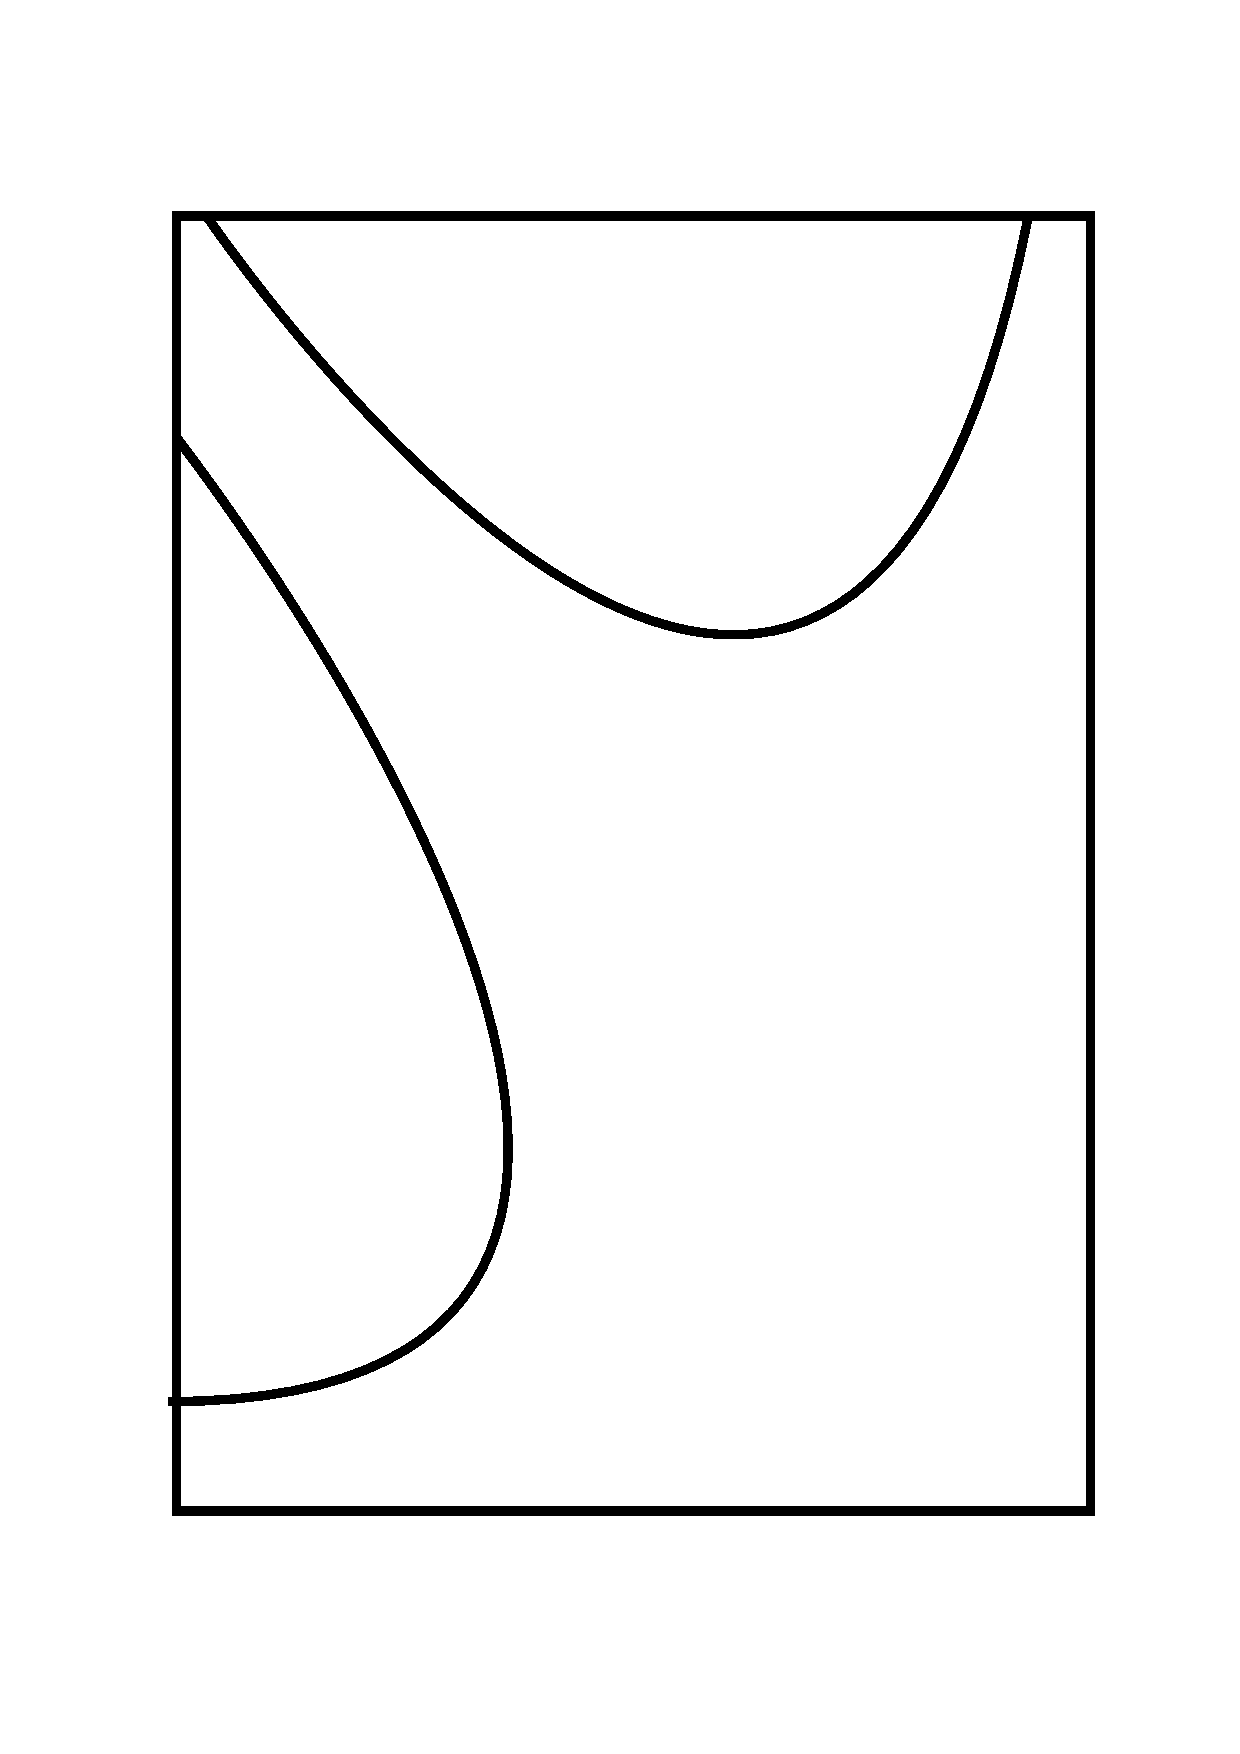
\includegraphics[width = 5cm]{2D1.pdf}
  \caption{2 Dimensions}
  \end{figure}
\end{columns}

\end{frame}

\begin{frame}
{\bf Bibliography}

\begin{itemize}
  \item Commodity price.
      \begin{itemize}
      \item Mean reversion:  Gibson and Schwartz (1990); Brennan and Hughes (1991); Cortazar and Schwartz (1994); Bessembinder, Coughenour, Seguin, Smoller (1995);
      \item Price Dyanmics: Schwartz (1997); Schwartz and Smith (2000);
      \end{itemize}
  \item Valuation of storage: \small{Fackler and Livingston (2002); Manoliu (2004); Hodges (2004); Chen and Forsyth (2008, 2010); Boogert and Jong (2008); Matt, Davison and Rasmussen (2009); Secomandi (2010, 2014); Zhao and Wijnbergen (2015)	}
  %No one model it as a singular control problem with non-trivial transaction cost.
  %No one used moving boundary method neither.
  
  \item Moving boundary method: \small{Muthuraman and Kumar (2006); Chockalingam and Muthuraman (2007, 2010, 2014); Muthuraman and Zha (2008); Feng and Muthuraman (2010); }
\end{itemize}

\end{frame}


\section{Model}
\begin{frame}
{\bf Model}
\begin{itemize}
  \item One factor model
\begin{equation*}
  dS_t = \kappa ( \mu - \ln S_t)S_t dt + \sigma S_t dW_t
\end{equation*}
\item By Ito's formula, $X_t = \ln(S_t)$ is an Ornstein-Uhlenbeck process,

\begin{equation*}
  dX_t = \kappa ( \alpha - X_t) dt + \sigma dW_t.
\end{equation*}

where $\alpha  = \gamma - \sigma^2/(2\kappa)$.
\end{itemize}

\end{frame}

\begin{frame}
{\bf Model}
\begin{itemize}
\item Storage level at time $t$ is $Q_t$. $L_t,U_t$ represent cumulative injections and withdrawals at time $t$.

\begin{equation*}
  dQ_t = dL_t - dU_t
\end{equation*}
\\
\item Admissible if $Q_t \in (Q_{min},Q_{max})~~ \forall t \geq 0$.

\item Costs of injection and withdrawal, $\lambda(X_t,Q_t)$ and $\mu(X_t,Q_t)$, are continuous and bounded.

%In the natural gas example, X_t: leak or use it as the energy for pump. Q_t difficulty.
\end{itemize}

\end{frame}


\begin{frame}
{\bf Model}
\begin{itemize}
  \item Objective: to maximize discounted infinite-horizon cash flows.

  \begin{equation}
  \begin{split}
  V(x,q) &= \max_{(L,U) \in \mathcal{U}} \mathbb{E}_{x,q} \left(\int_{0}^{\infty} e^{-\beta t}(e^{X_t} - \mu(Q^1_t))dU_t\right.\\
  &\left.- \int_{0}^{\infty}e^{-\beta t}(e^{X_t} + \lambda(Q^2_t))dL_t\right)
  \end{split}
\end{equation}
% I need to mention this.
where $X_0 =x$ and $Q_0 = q$. %What's more,
%\begin{equation}
%\begin{split}
%  \mu(Q^1_t) = \frac{1}{U_t - U_{t-}}\int_{U_{t-}}^{U_t} \mu(q) dq
%  \end{split}
%\end{equation}
%
%\begin{equation}
%  \lambda(Q^2_t) = \frac{1}{L_t - L_{t-}}\int_{L_{t-}}^{L_t} \lambda(q) dq.
%\end{equation}  
  
\end{itemize}
\end{frame}

\begin{frame}
{\bf The Hamilton-Jacobi-Bellman Equation}
\begin{itemize}
  \item Dynamic programming arguments and Ito's formula yield the Hamilton-Jacobi-Bellman (HJB) equation.
  \begin{equation*}
  \max\left( \mathcal{L} V, \frac{\partial V}{\partial q} - (e^x + \lambda(q)), -\frac{\partial V}{\partial q} + (e^x - \mu(q))\right) = 0
\end{equation*}
with $\mathcal{L}V = \frac{1}{2} \sigma^2 \frac{\partial^2 V}{\partial x^2} + \alpha (\kappa - x) \frac{\partial V}{\partial x} - \beta V$.


  \item A verification theorem assures us that a function that solves the HJB equation is the value function for the original control problem and a policy that achieves this value function is the optimal policy.

\end{itemize}

\end{frame}

\begin{frame}
{\bf The Hamilton-Jacobi-Bellman Equation}
%The first part is the discounted value earned in the future while the second part is the cost I need to pay right now.

\begin{itemize}
\item Assume $V$ is known and the change of policy at one point $(x_0,q_0)$ won't affect it.\\
Now at $(x_0,q_0)$, $\epsilon$ is bought at price $e^{x_0}$. The average buying profit is 
\begin{equation*}
  \frac{\left[V(x_0,q_0 + \epsilon) - V(x_0,q_0)\right] - \epsilon(e^x + \lambda(q))}{\epsilon}
  \stackrel{\epsilon \rightarrow 0}{\longrightarrow} 
  \frac{\partial V}{\partial q} - (e^x + \lambda(q))
\end{equation*}

\item $\mathcal{L}V(x,q)$: holding profit at $(x,q)$.
\item $\frac{\partial V}{\partial q}(x,q) - (e^x + \lambda(q))$: selling profit at $(x,q)$.
\item $-\frac{\partial V}{\partial q}(x,q) + (e^x - \mu(q))$: buying profit at $(x,q)$.

\item HJB equation.
\begin{equation*}
  \max\left( \mathcal{L} V, \frac{\partial V}{\partial q} - (e^x + \lambda(q)), -\frac{\partial V}{\partial q} + (e^x - \mu(q))\right) = 0
\end{equation*}



\end{itemize}

\end{frame}


\begin{frame}
{\bf Holding, Selling and Buying Regions}

\begin{itemize}
  \item The state space $(x,q) \in \mathbb{R}^2_+$ is divided into three kinds of regions.
  \item {\small Holding region $H^*$: holding profit = 0, selling \& buying profit $<0$}
  \item {\small Selling region $S^*$: selling profit = 0, holding \& buying profit $<0$}
  \item {\small Buying region $B^*$: buying profit = 0, holding \& selling profit $<0$}
\end{itemize}

\end{frame}

\section{Moving Boundary Method}
\begin{frame}
{\bf Moving Boundary Method}
\only<1>{
	\begin{itemize}
	  \item Start with an initial guess and iteratively improve it until convergence.\\
	  \item A sequence of fixed boundary problems $\rightarrow$ free boundary problem\\
	\end{itemize}
}
\only<2>{
	\begin{itemize}
		\item Initial guess.
		\item How to solve fixed boundary problems efficiently.
		\item How to improve boundary.
	\end{itemize}
}


\end{frame}

\begin{frame}
{\bf Initial Guess}

\begin{theorem}
When the price is high enough, regardless of storage, selling is the optimal strategy.
\end{theorem}

% The initial guess for selling boundary is easy. At a high price, set the policies at that level are selling.
% Give an counter example of second intuition.

\end{frame}

\begin{frame}
{\bf Solving the Fixed Boundary Problem}
\begin{itemize}
  \item In the holding region
  \begin{equation*}
  \frac{1}{2} \sigma^2 \frac{\partial^2 V}{\partial x^2} + \alpha (\kappa - x) \frac{\partial V}{\partial x} - \beta V = 0
\end{equation*}

\item Defining $y = \kappa (x-\alpha)^2/\sigma^2$, we have
\begin{equation*}
  y \frac{\partial^2 V}{\partial y^2} + (0.5 - y) \frac{\partial V}{\partial y} -\frac{\beta}{2\kappa} V = 0
\end{equation*}

which is the Kummer Equation. The solution is the sum of hypergeometric1F1 and the hypergeometricU functions.

\begin{equation*}
\begin{split}
  V(x,q) &= A(q)\text{HyperGeoU}\left(\frac{\beta}{2\kappa},\frac{1}{2},\frac{\kappa}{\sigma^2}(x-\alpha)^2\right) \\
  &+ B(q)\text{HyperGeo1F1}\left(\frac{\beta}{2\kappa},\frac{1}{2},\frac{\kappa}{\sigma^2}(x-\alpha)^2\right)
  \end{split}
\end{equation*}

Boundary conditions can determine $A(q)$ and $B(q)$.

\end{itemize}

\end{frame}

\begin{frame}
{\bf Boundary Movement}

\begin{columns}
   \column{0.4\textwidth} 

\begin{itemize}
  \item Direction.
  \item Distance.
\end{itemize}

  \column{0.7\textwidth}
\only<2>{\begin{figure}[hbt]
  \includegraphics[scale = 0.4]{0step.eps}
  \caption{Initial Guess}
  \end{figure}}
\only<3>{\begin{figure}[hbt]
  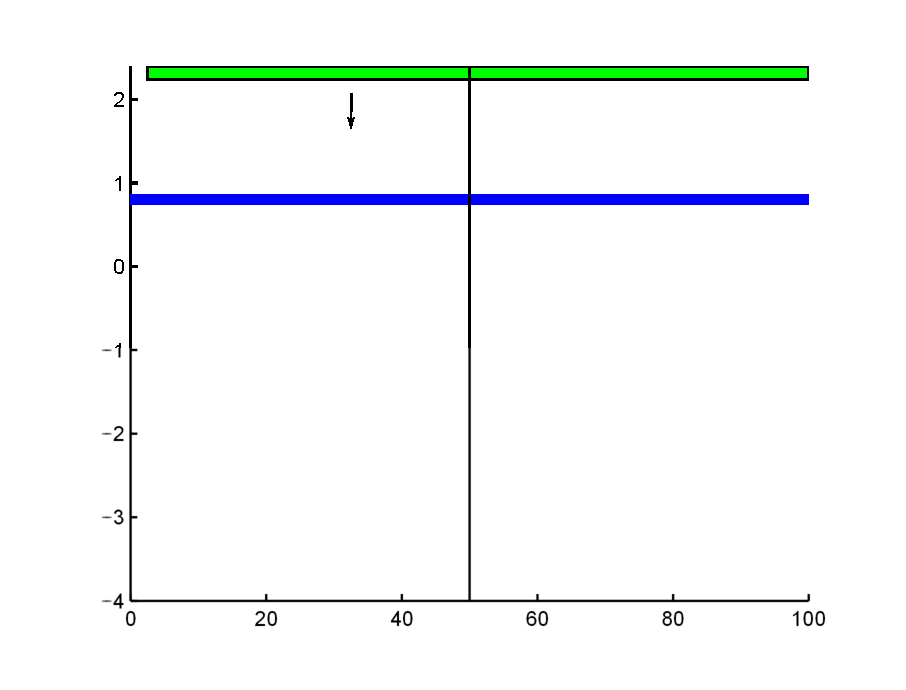
\includegraphics[scale = 0.4]{Where2Move0step.eps}
  \caption{Initial Guess}
\end{figure}}
  \end{columns}
\end{frame}




%\begin{frame}
%{\bf How does Moving Boundary Method Work?}
%
%%todo: use movie instead of pictures to show this. At first show it extremely slow then increase the speed toward the end.
%\centering
%\only<1>{
%\begin{figure}[hbt]
%  \includegraphics[scale = 0.5]{0step.eps}
%  \caption{Initial Policy}
%\end{figure}
%}
%
%%%\only<2>{
%%%\begin{figure}[hbt]
%%%  \includegraphics[scale = 0.5]{1step.eps}
%%%  \caption{1st Step}
%%%\end{figure}
%%%}
%%%\only<3>{
%%%\begin{figure}[hbt]
%%%  \includegraphics[scale = 0.5]{2step.eps}
%%%  \caption{2nd Step}
%%%\end{figure}
%%%}
%%%\only<4>{
%%%\begin{figure}[hbt]
%%%  \includegraphics[scale = 0.5]{3step.eps}
%%%  \caption{3rd Step}
%%%\end{figure}
%%%}
%
%\only<2>{
%\begin{figure}[hbt]
%  \includegraphics[scale = 0.5]{9step.eps}
%  \caption{9th Step}
%\end{figure}
%}
%
%\only<3>{
%\begin{figure}[hbt]
%  \includegraphics[scale = 0.5]{10step.eps}
%  \caption{10th Step}
%\end{figure}
%}
%
%\only<4>{
%\begin{figure}[hbt]
%  \includegraphics[scale = 0.5]{11step.eps}
%  \caption{11th Step}
%\end{figure}
%}
%
%\only<5>{
%\begin{figure}[hbt]
%  \includegraphics[scale = 0.5]{12step.eps}
%  \caption{12th Step}
%\end{figure}
%}
%
%\only<6>{
%\begin{figure}[hbt]
%  \includegraphics[scale = 0.5]{13step.eps}
%  \caption{13th Step}
%\end{figure}
%}
%
%\only<7>{
%\begin{figure}[hbt]
%  \includegraphics[scale = 0.5]{14step.eps}
%  \caption{14th Step}
%\end{figure}
%}
%
%\only<8>{
%\begin{figure}[hbt]
%  \includegraphics[scale = 0.5]{laststep.eps}
%  \caption{Last Step}
%\end{figure}
%}
%
%\end{frame}

\begin{frame}
{\bf Distance}


{\large Sell}
\begin{columns}
\column{0.5\textwidth}
%\only<1>{
\begin{figure}[hbt]
  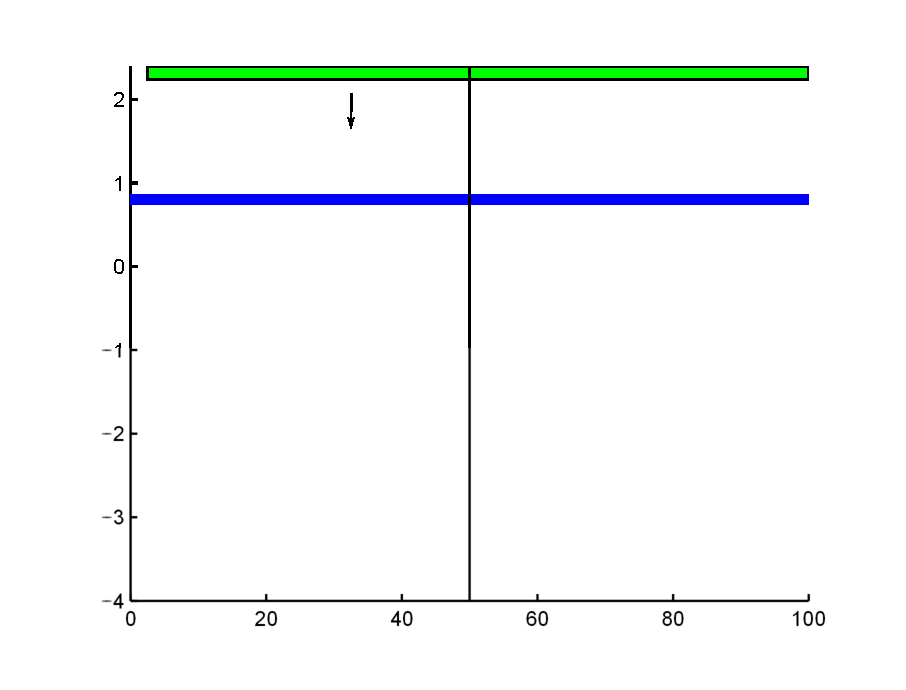
\includegraphics[scale = 0.4]{Where2Move0step.eps}
  \caption{Current Policy}
\end{figure}
%}
  \column{0.5\textwidth} 
  \only<2>{
\begin{figure}[hbt]
  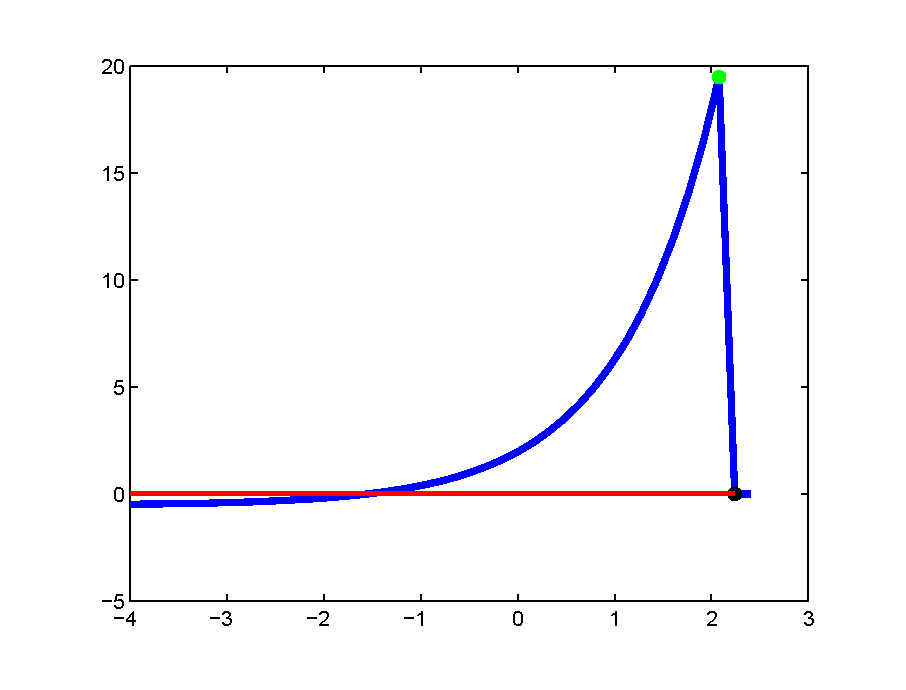
\includegraphics[scale = 0.4]{Where2MoveSell.eps}
  \caption{Selling Profit}
\end{figure}
}
\only<3>{
\begin{figure}[hbt]
  \includegraphics[scale = 0.4]{Where2Move1step.eps}
  \caption{After Movement}
\end{figure}
}
\end{columns}
\end{frame}

\begin{frame}

{\large Buy}
%todo: put a black dot in the graph and an arrow there.
\begin{columns}
\column{0.5\textwidth}
%\only<1>{
\begin{figure}[hbt]
  \includegraphics[scale = 0.4]{Where2Move13step.eps}
  \caption{Current Policy}
\end{figure}
%}
  \column{0.5\textwidth} 
\only<2>{
\begin{figure}[hbt]
  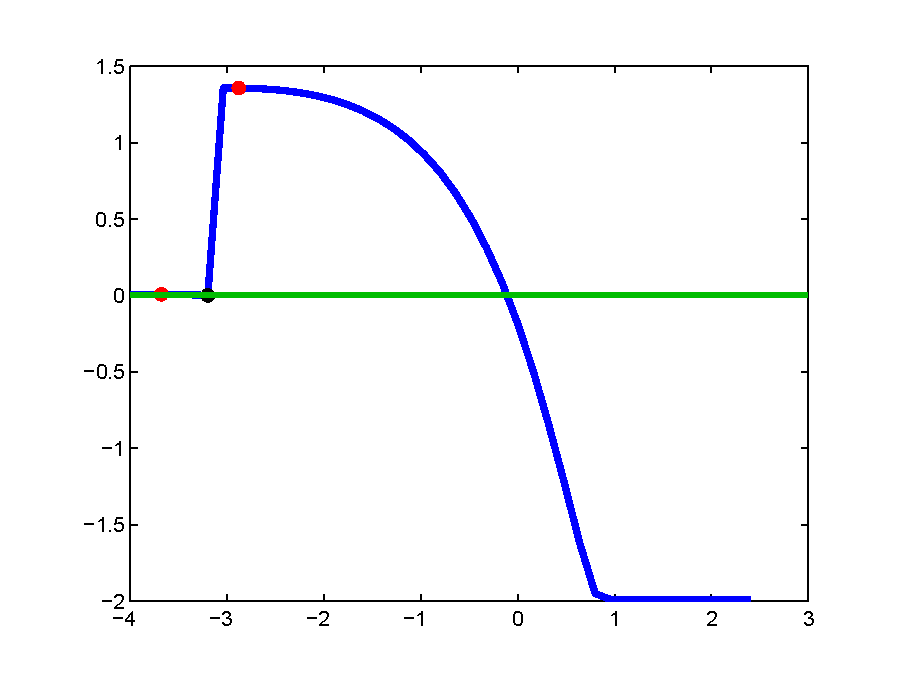
\includegraphics[scale = 0.4]{Where2MoveBuy.eps}
  \caption{Buying Profit}
\end{figure}
}
\only<3>{
\begin{figure}[hbt]
  \includegraphics[scale = 0.4]{Where2Move14step.eps}
  \caption{After Movement}
\end{figure}
}
\end{columns}
\end{frame}

\begin{frame}
{\bf Algorithm}
\begin{enumerate}
  \item Begin with selling at very high price for all $q>0$.
  \item Move selling (buying) boundary along price $x$ to local maximal selling (buying) profit points until convergence. 
%  \begin{itemize}ss
%  \item  The initial guess of buying is generated in this procedure.
%  \item  Each time move to the point that generates highest positive profit.
%\end{itemize}
\end{enumerate}

\end{frame}


\begin{frame}
{\bf Proof of Convergence}
\begin{Theorem}
Each movement improves value function.
\end{Theorem}
\begin{columns}
   \column{0.6\textwidth} 
   \small{
   \only<1>{
		\begin{equation*}
		\begin{array}{ll}
		\LL V^{n}(x,q) = 0& H^{n}\\
		-V^{n}_q(x,q) + e^x - \mu(q) = 0 & S^{n}\\
		V^{n}_q(x,q) - e^x - \lambda(q) = 0 & B^{n}\\
		-V^{n}_q(x,q) + e^x - \mu(q) > 0 & S^{n+1}/S^{n}\\
		V^{n}_q(x,q) - e^x - \lambda(q) > 0 & B^{n+1}/B^{n}\\
		\end{array}
		\end{equation*}
	}

	\only<2>{
		\begin{equation*}
		\begin{array}{ll}
		\LL V^{n+1}(x,q) = 0 & H^{n+1}\\
		-V^{n+1}_q(x,q) + e^x - \mu(q) = 0 & S^{n+1}\\
		V^{n+1}_q(x,q) - e^x - \lambda(q) = 0 &  B^{n+1}\\
		\end{array}
		\end{equation*}
	}

	\only<3>{
		\begin{equation*}
		\begin{split}
		\LL \Delta V^{n+1}(x,q) &= 0 \quad H^{n+1}\\
		\Delta V_q^{n+1}(x,q) &= 0 \quad S^{n}\\
		\Delta V_q^{n+1}(x,q) &> 0 \quad S^{n+1}/S^{n}\\
		\Delta V_q^{n+1}(x,q) &= 0 \quad B^{n}\\
		\Delta V_q^{n+1}(x,q) &< 0 \quad B^{n+1}/B^{n}\\
		\end{split}  
		\end{equation*}
	}
	
	\only<4>{
		\begin{equation*}
		\begin{split}
		\LL \Delta V^{n+1}(x,q) &= 0 \quad H^{n+1}\\
		\Delta V_q^{n+1}(x,q) &\geq 0 \quad S^{n+1}\\
		\Delta V_q^{n+1}(x,q) &\leq  0 \quad B^{n+1}\\
		\end{split}  
		\end{equation*}
	}
	
	}
	\column{0.5\textwidth}
	\begin{figure}[hbt]
	  \includegraphics[scale = 0.4]{PolicyImproveValue1.pdf}
	\end{figure}
\end{columns}

\end{frame}

%Todo: give more intuition about this theorem. Make sure with Kumar that this is the right way.

\begin{frame}
{\bf Proof of Convergence}
% What does \Delta V_q > 0 mean?
\begin{Theorem}
The boundaries can be kept moving.
\end{Theorem}

\begin{columns}
   \column{0.6\textwidth} 
   \small{

	\only<1>{
		\begin{equation*}
		\begin{split}
		\LL \Delta V^{n+1}(x,q) &= 0 \quad H^{n+1}\\
		\Delta V_q^{n+1}(x,q) &= 0 \quad S^{n}\\
		\Delta V_q^{n+1}(x,q) &> 0 \quad S^{n+1}/S^{n}\\
		\Delta V_q^{n+1}(x,q) &= 0 \quad B^{n}\\
		\Delta V_q^{n+1}(x,q) &< 0 \quad B^{n+1}/B^{n}\\
		\end{split}  
		\end{equation*}
	}
	
	\only<2>{
	At upper point
		\begin{equation*}
		\begin{split}
		& (\Delta V_q^{n+1}(x,q))_x  \leq 0 \\
		& (- V_q^{n}(x,q) + (e^x - \mu(q)))_x  =  0\\
		\Rightarrow &(- V_q^{n + 1}(x,q) + (e^x - \mu(q)))_x  \leq  0\\
		\end{split}  
		\end{equation*}
	}
	
	}
	\column{0.5\textwidth}
	\begin{figure}[hbt]
	  \includegraphics[scale = 0.4]{PolicyImproveValue2.pdf}
	\end{figure}
\end{columns}

\end{frame}


\begin{frame}
{\bf Extensions}

\begin{itemize}
  \item Seasonality.
\end{itemize}

\end{frame}




\end{document} 